\scanpage{236}
\mspage{186}
% L1–4, continuation at head
peut-être une attention particulière, car on
ne sait pas \unsure{$=$} encore que $Z$ est $1$-connexe.
Mais \deleted{\unsure{par}} on sait que $c_2$ implique $c_1$, qui équivaut
à $b_1$, \unsure{donc on a}
% L5–9, three successive maps
\[
 \pi_1(X,x)\longrightarrow\pi_1(Y,y)\qquad\text{iso,}
\]
donc
\[
 \pi_1(Z,x)\unsure{-|\to}\pi_1(X,x)\qquad\text{\uline{nul}}
\]
donc
\[
 \pi_2(Y,y)\unsure{-|\to}\pi_1(Z,x)\qquad\text{épi,}
\]
% L10–14, condition on the first homotopy group
ce qui implique tout au moins que
$\pi_1(Z,\unsure{x|z})$ est \uline{abélien}. \deleted{\unsure{Donc il}} Il faut le
voir comme un $\pi$-Module, et prouver
sa nullité comme tel (moyennant $c_2$).

% L15–19, general case and spectral sequence
Passons au cas général. On a pour $F$ loc
constant abélien sur $Y$
\[
 H^*(X,F_X)\Longleftarrow
 \underbrace{E_2^{pq}\unsure{=|\Leftarrow|\ne}H^p(Y,H^q(Z,F_Z))}
 _{\substack{=0\ \text{si }0<q<n-1\\\text{car }Z\text{ est }(n-2)\text{-connexe}.}}
\]
% L20, small diagram at right
\figure{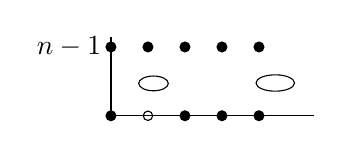
\begin{tikzpicture}[x=.47cm,y=.52cm]
 \draw (0,1.93)--(0,0)--(5.5,0);
 \node[left] at (0,1.68) {$n-1$};
 \foreach \x in {0,1,2,3,4} {\fill (\x,1.68) circle (2pt);}
 \foreach \x in {0,2,3,4} {\fill (\x,0) circle (2pt);}
 \draw (1,0) circle (1.7pt);
 \draw (1.15,.79) ellipse (.40 and .18);
 \draw (4.44,.80) ellipse (.52 and .20);
\end{tikzpicture}}
% L21–23, descending sequence at the foot
D'où
\[
 \begin{aligned}
 \scriptstyle 0\longrightarrow H^{\unsure{n-1|n}}(Y,F)\longrightarrow H^{n-1}(X,F_X)
 &\scriptstyle\longrightarrow\underbrace{H^0(Y,H^{n-1}(Z,F_Z))}
 _{\substack{\operatorname{Hom}_\pi(\pi_{n-1}(Z;x),F_x)\\\text{par Hurwicz}}}
 \\
 &\quad\searrow H^n(Y,F)\\
 &\qquad\qquad\searrow H^n(X,F_{\unsure{x|X}}\unsure{)}
 \end{aligned}
\]
% L24, unfinished at the lower edge
L'hypothèse $c_n$ implique qu'on a
% archive sheet number: 236
